\section{Divide et Impera}
Il metodo Divide et Impera, non ha memoria, ogni volta che si calcola una soluzione, il processo richiede di ricalcolare la sottoistanza del problema che lo ha risolto, generando quindi un problema di sottoistanze ripetute. \\~\\

Il Divide et Impera, possiede 2 fasi:
\begin{itemize}
    \item \textbf{Top-down:} con cui vengono generate le istanze risolte divide il problema originale in un numero di sottoproblema (divide), risolvendo i problemi ricorsivamente (impera) e combinando le soluzioni dei sottoproblemi nella soluzione ai sottoproblemi originali (combine)
    \item \textbf{Bottom-up:} normalmente non ricorsiva ma iterativa
    \begin{itemize}
        \item caratterizza la struttura delle soluzioni ottimali
        \item definiscono ricorsivamente i valori delle soluzioni ottimali
        \item calcola il valore delle soluzioni ottimali
        \item costruisce una soluzione ottimale a partire dalle informazioni calcolate
    \end{itemize}
    Sinteticamente, si elaborano le soluzioni alle istanze presenti.
\end{itemize}
\begin{center}
    \begin{tabular}{c}
        \\ 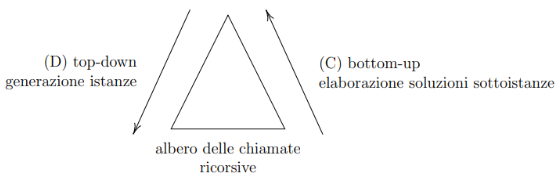
\includegraphics[width=0.8\textwidth]{image/T-D_B-U.png} \\ \\
    \end{tabular}
\end{center}
L'approccio della programmazione dinamica salta completamente l'approccio top-down, normalmente usando algoritmi iterativi per evitare di dover calcolare la soluzione. La programmazione Divide et Impera usa entrambi gli approcci e normalmente in modo ricorsivo.
